% !TEX root = morphkasten.tex

\section{Rechtsvortritt}


%##############
\subsection{Sensor}

Grafik

\begin{table}[h]
\begin{tabular}{p{0.5\textwidth} | p{0.5\textwidth}}


 \textbf{Vorteile} & \textbf{Nachteile} \\ \hline
	 
\begin{itemize}
\item Vorteil 1
\item Vorteil 2
\item Vorteil 3
\item ...
\end{itemize}

 
 &
 
\begin{itemize}
\item Nachteil 1
\item Nachteil 2
\item Nachteil 3
\item ...
\end{itemize}

\end{tabular}
\end{table}

\begin{table}[h]
\begin{tabular}{p{0.5\textwidth}p{0.5\textwidth}}


 \textbf{Risiken} & \\ \hline
	 
\begin{itemize}
\item Risiko 1
\item Risiko 2
\end{itemize}
&
\begin{itemize}
\item Risiko 3
\item ...
\end{itemize}

 
\end{tabular}
\end{table}

\pagebreak


%##############
\subsection{Bilderkennung}

\begin{figure}[h!]%Position festigen
\centering
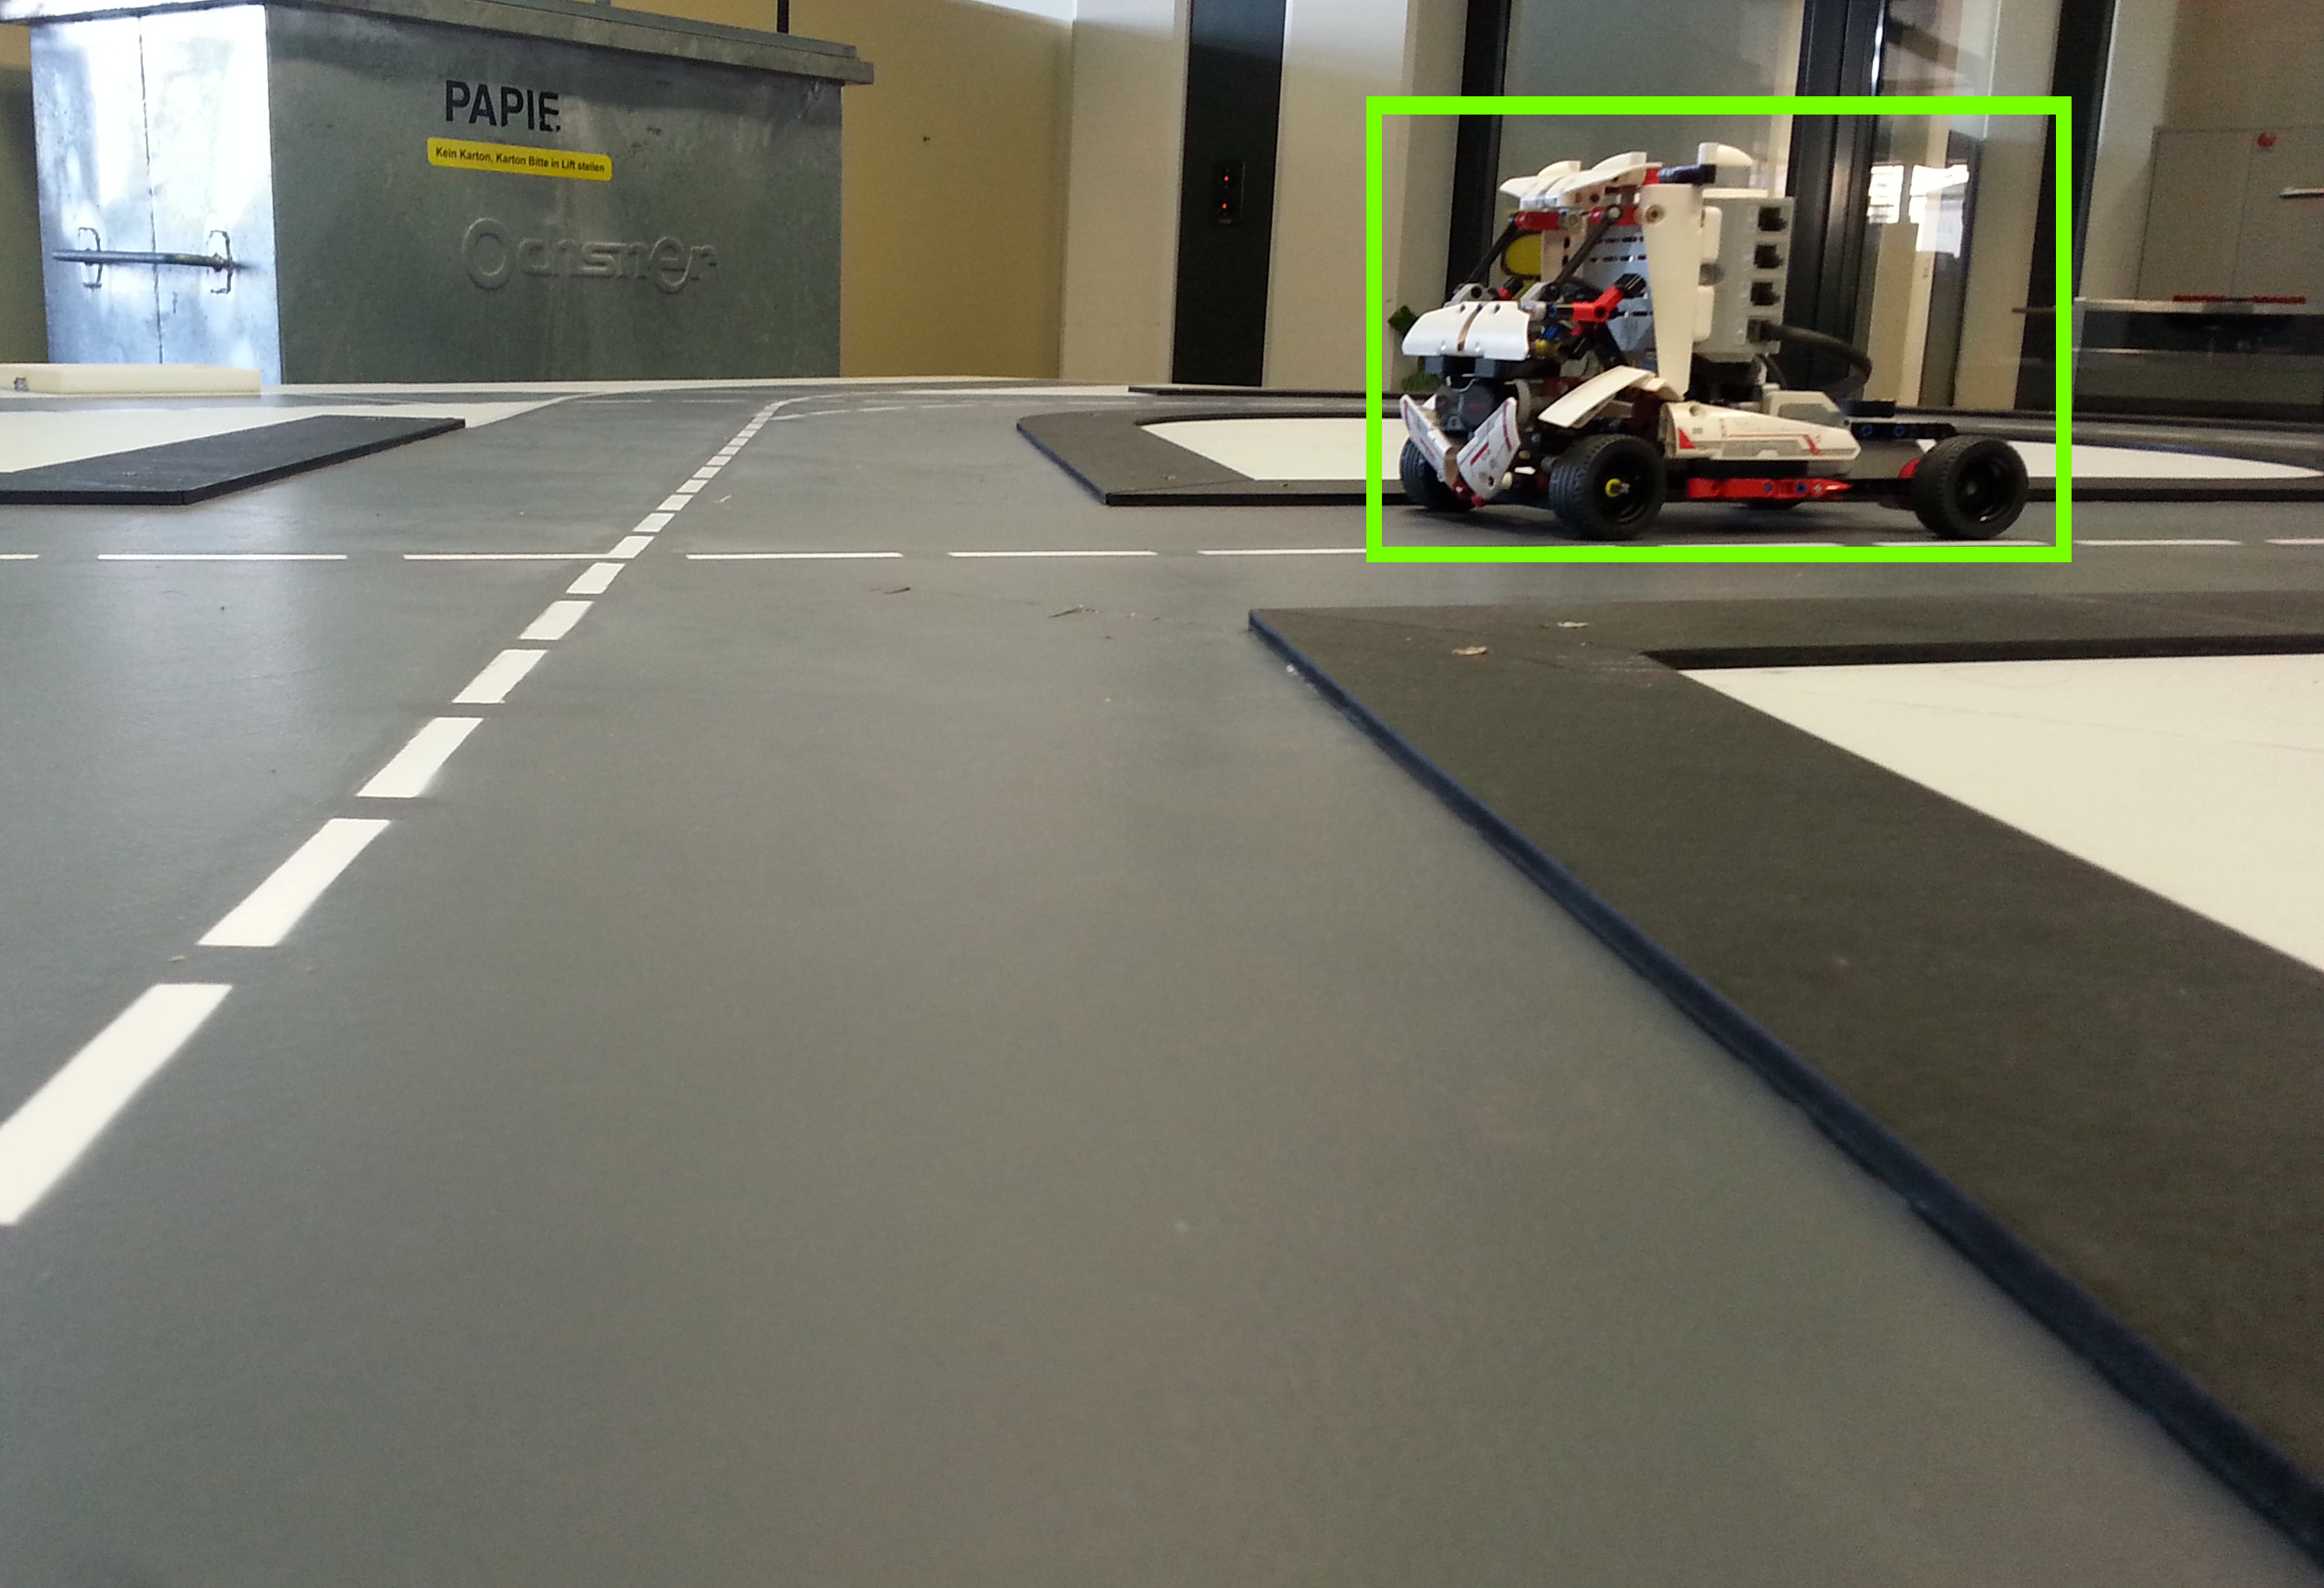
\includegraphics[width=0.7\textwidth]{fig/rechtsvortritt_bilderkennung.png}
\caption{Bilderkennung Rechtsvortritt}
\label{fig:Bilderkennung Rechtsvortritt}
\end{figure}

\begin{table}[h]
\begin{tabular}{p{0.5\textwidth} | p{0.5\textwidth}}


 \textbf{Vorteile} & \textbf{Nachteile} \\ \hline
	 
\begin{itemize}
\item Stoppen durch Vorausplnung möglich
\item Unterschiede berechnen, wie sich das andere Fahrzeug bewegt
\end{itemize}

 
 &
 
\begin{itemize}
\item Genaue Definition, was ein Fahzeug an der Kreuzung beim Rechtsvortritt ist
\item rechenintensiv
\end{itemize}

\end{tabular}
\end{table}

\begin{table}[h]
\begin{tabular}{p{0.5\textwidth}p{0.5\textwidth}}


\textbf{Risiken} & \\ \hline
	 
\begin{itemize}
\item Fahrzeug wird auch an anderen Stellen erkennt
\item andere Gegenstände könnten als Fahrzeug interpretiert werden

\end{itemize}

 
\end{tabular}
\end{table}

\pagebreak